%%% Dario Chinelli 24/05/21

\section{Decadimenti nucleari}
La formula semi-emipirica di massa, equazione \ref{formula_semiempirica_massa} nei capitoli precedenti, esprime la stabilità o instabilità dei nuclei nel caso in cui ci sia un'abbondanza di neutroni o di protoni.
Per basi numeri atomici il numero di protoni e di neutroni si equivale, aumentando il numero di massa i nuclei tendono ad avere più neutroni che protoni ed in particolare i nuclei stabili e arrivano ad un numero atomico di circa 80 ed un numero di neutroni di circa 110.
Tutti gli atomi con elevato numero atomico e di massa sono instabili, come ad esempio l'uranio che ha numero atomico 92 ed è un elemento instabile che si trova in natura.
Il decadimento dei nuclei avviene spontaneamente in alcune circostanze
\begin{figure}[h]
\centering
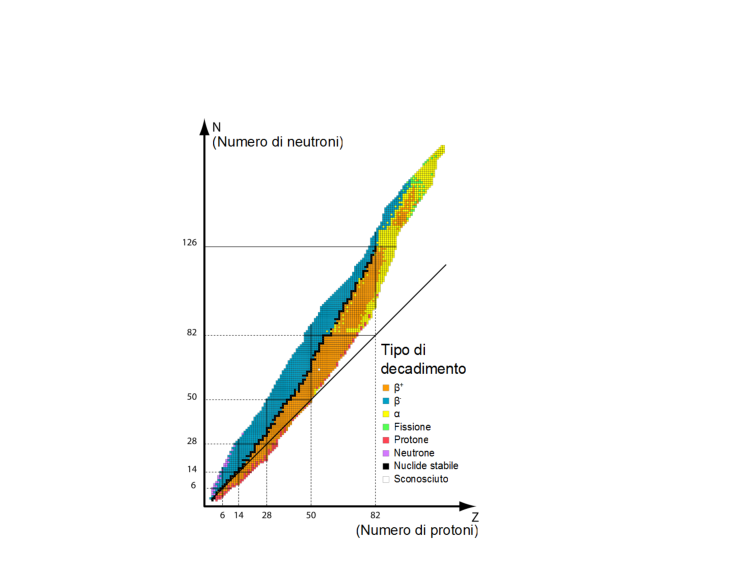
\includegraphics[scale=1]{/nuclei_stabili}
\caption{Il grafico rappresenta per quali combinazioni di neutroni e protoni si hanno atomi stabili.}
\end{figure}
\begin{enumerate}
\item  il nucleo ha troppi neutroni, allora si ha un processo di decadimento beta $\beta^-$
\begin{equation}
^{A}_{Z}X \quad\longrightarrow\quad  ^{A}_{Z+1}Y + e^- + \bar\nu_e
\end{equation}
dopo il decadimento si ha un atomo di una diversa specie atomica.
\item il nucleo può avere troppi protoni, si ha allora un processo di decadimento beta $\beta^+$
\begin{equation}
^{A}_{Z}X \quad\longrightarrow\quad ^{A}_{Z-1}Y + e^+ + \nu_e
\end{equation}
dopo il decadimento si ha un atomo di una diversa specie atomica.
\item se ci sono troppi nucleoni, quindi siamo nella parte alta del grafico, i nuclei tendono a subire un processo di decadimento alpha $\alpha$, una particella alpha è un nucleo di Elio
\begin{equation}
^{A}_{Z}X \quad\longrightarrow\quad ^{A-4}_{Z-2}Y + \alpha
\end{equation}
\item il nucleo potrebbe avere anche troppa energia, quindi nel caso di un nucleo eccitato $X^{\ast}$, si ha emissione di radiazione elettromagnetica chiamata \emph{radiazione gamma}
\begin{equation}
^{A}_{Z}X^{\ast} \quad\longrightarrow\quad ^{A}_{Z}X + \gamma
\end{equation}
\item nel caso in cui le energie di eccitazione siano molto elevate si può avere decadimento per \emph{fissione} 
\end{enumerate}
Le leggi che descrivono un decadimento impongono la conservazione di 
\begin{itemize}
\item energia
\item quantità di moto
\item carica elettrica
\item numero di nucleoni
\item numero di leptoni
\end{itemize}
la massa invece non si conserva nei processi di decadimento.

\paragraph{esempio} utilizzando la formula semi-empirica di massa si verifichi se il decadimento $\alpha$ del $^{238}_{92} U$ sia possibile energeticamente.

La massa totale iniziale del sistema deve essere maggiore della massa totale finale, allora il processo è esotermico.
$$ M_i > M_f \quad\Rightarrow\quad esotermico $$
\begin{equation}
^{238}_{92} U \quad\longrightarrow\quad ^{234}_{90}X + ^{4}_{2}He
\end{equation}
(l'elemento figlio di questa reazione è un isotopo del Torio $^{232}_{90}Th$, ma non è importante ai fini della trattazione)
dobbiamo calcolare il $Q$ della reazione e ci chiediamo se è maggiore di zero
\begin{equation}
Q = M(A,Z) - M(A-4,Z-2) - M(^{4}_{2}He^{++}) > 0
\end{equation}
la massa dell'atomo iniziale equivale a
\begin{equation}
M(A,Z) = Z M_H + (A-Z)M_n - B(A,Z)
\end{equation}
dove $B$ rappresenta l'energia di legame
quindi il calore nella reazione è
\begin{equation}
\begin{split}
Q  & = -B(A,Z) + B(A-4,Z-2) + B(^{4}_{2}He^{ ++ }) \\
& = [ -1807.5 + (1784 + 32.85)] MeV = \SI{9.35}{MeV} > 0
\end{split}
\end{equation}
risulta quindi positivo, per cui il decadimento alpha è energeticamente possibile, anzi avviene spontaneamente; questo calcolo non ci dice nulla però sulla probabilità che avvenga.
La natura tende a minimizzare la massa.

Ci si può divertire con un programma in MathLab delle slide calcolando l'energia di legame per tutti i nuclei...
si trova l'andamento del calore Q emesso/assorbito dalla reazione in funzione del numero atomico, vedi figura \ref{calore_vs_numatomico}
\begin{figure}[h]
\centering
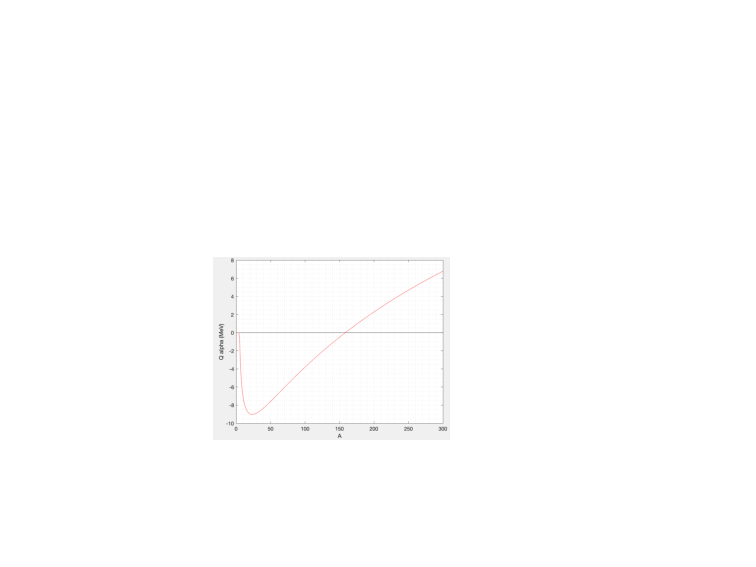
\includegraphics[scale=3]{/calore_vs_numatomico}
\caption{Andamento del calore in funzione del numero atomico}
\label{calore_vs_numatomico}
\end{figure}

\paragraph{esempio} si verifichi se l'Uranio $^{238}_{92}U$ possa decadere $\beta^-$
\begin{equation}
^{238}_{92}U \quad\longrightarrow\quad ^{238}_{92}U + ^{238}_{93}U + e^- + \bar\nu_e
\end{equation}
ovvero ci si chiede se il calore della reazione è maggiore di zero
\begin{equation}
\begin{split}
Q & = M(A,Z) - M(A,Z+1) \quad\quad > 0 \quad ? \\
& = -B(A,Z) + B(A,Z+1) + (M_H - M_n) \\
& = -1807.5 + 1805 + (-0.78) = - \SI{3.28}{MeV} < 0
\end{split}
\end{equation}
l'uranio non decade spontaneamente $\beta^-$.


\subsection{Legge del decadimento radioattivo}
Il numero di decadimenti al secondo è proporzionale al numero di atomi contenuti nel campione.
$$\frac{decad}{s} \propto atom$$
Introduco la \emph{costante di decadimento} $\lambda$, che mi permette di riscrivere la formula precedente come
\begin{equation}
\frac{dN}{dt} = - \lambda N
\end{equation}
questa è un'equazione differenziale risolvibile tramite separazione delle variabili, che descrive la probabilità che un atomo decada nell'unità di tempo
\begin{equation}
\begin{split}
\frac{dN}{N} & = - \lambda dt \\
\ln N & = -\lambda t + C \\
N & = e^{-\lambda t + C} = e^{-\lambda t } e^C 
\end{split}
\end{equation}
trovo la costante di integrazione $C$, imponendo che al tempo $t=0$ il numero totale di atomi sia $N=N_0$,
quindi ottengo $N_0 = 1 e^C$, da cui scriverò
\begin{equation}
N = N_0 e^{-\lambda t} 
\label{eq_decad}
\end{equation}

Il decadimento viene descritto anche da altre quantità, come il \emph{tempo di dimezzamento} $T_{1/2}$: cioè il tempo dopo il quale il numero di neuclidi iniziali si è dimezzato, ovvero $N = N_0 / 2$ e quindi $t= T_{1/2}$
\begin{equation}
\begin{split}
& \frac{N_0}{2} = N_0 e^{-\lambda T_{1/2}} \\
& 2 = e^{ \lambda T_{1/2} } \\
& T_{1/2} = \frac{\ln 2}{\lambda} \simeq \frac{0.693}{\lambda}
\end{split}
\end{equation}
questo tipo di decadimento esponenziale è un processo puramente quantistico, un essere vivente non ha questi problemi... (lol)

Un'altra quantità importante è detta \emph{vita media} $\tau$: 
\begin{equation}
\begin{split}
\tau & = \frac{\int_{N_0}^{0} t dN}{N_0}  = \frac{1}{N_0} \int_0^{\infty} t (-\lambda N_0 e^{ -\lambda t })dt \\
& = - \lambda \Bigl[  \frac{t (-e^{-\lambda t})}{\lambda} - \int \frac{(1) (-e^{ -\lambda t })}{\lambda} \Bigr]_0^{\infty} \\
& = - \lambda \Bigl[  \frac{- t e^{-\lambda t}}{\lambda} - \frac{ e^{ -\lambda t }}{\lambda^2} \Bigr]_0^{\infty} \\
& = \frac{1}{\lambda}
\end{split}
\end{equation}
per cui la vita media corrisponde all'inverso della costante di decadimento e anche a
\begin{equation}
\tau = \frac{1}{\lambda} = \frac{T_{1/2}}{\ln 2} = 1.44 \cdot T_{1/2}
\end{equation}
che corrisponde al momento in cui il numero di neuclidi è sceso al $37\%$ rispetto al valore iniziale.

È da notare che essendo questo un fenomeno quantistico è quindi anche casuale, ciò che sappiamo è che \emph{mediamente} decadono una certa quantità di nuclei ma non sappiamo quali ne quando succederà.
Il tempo di decadimento è indipendente dalla vita del nucleo, per cui esso può decadere immediatamente oppure non decadere mai. 
Ciò differisce nettamente dallo studio di sistemi biologici, che seguono regole più deterministiche.
Seguendo la \ref{eq_decad}, se ci si aspetta $\Delta N $ eventi in un secondo, tale numero di eventi potrà variare, statisticamente rispetto alla media, seguendo la statistica di Poisson in un intervallo dato da
\begin{equation}
\Delta N - \sqrt{\Delta N} < \Delta N < \Delta N + \sqrt{\Delta N}
\end{equation}
nel $67\%$ dei casi il numero di decadimenti sarà compreso in questo intervallo, ma non è una grandezza deterministica.

\paragraph{esempio} supponiamo di avere $10^{12}$ nuclei con una vita media di $\tau = \SI{e10}{s}$, 
quanti decadimenti si hanno in un secondo?
\begin{equation}
\frac{10^{12}}{10^{10}} - \sqrt{\frac{10^{12}}{10^{10}} } < \Delta N < \frac{10^{12}}{10^{10}} + \sqrt{\frac{10^{12}}{10^{10}} } \quad\Rightarrow\quad 90 < \Delta N < 110
\end{equation}
abbiamo in questo caso una precisione del $10\%$.

Nei processi di decadimento molto rari si utilizza la statistica di Poisson.
\paragraph{esempio} se ho $\Delta n$ al secondo che probabilità ho di registrare $K$ eventi? (se $\Delta n$ è piccolo, con bassa costante di decadimento) la probabilità in questo caso è data dalla statistica di Poisson
\begin{equation}
P(\Delta n, K) = \frac{\Delta n^K}{K!} e^{ -\Delta n }
\end{equation}

\subsection{Catene di decadimento}
Normalmente i decadimenti avvengono in cascata e sono dominate da un sistema di equazioni differenziali, tali equazioni sono chiamate \emph{equazioni di Bateman}
\begin{equation}
\begin{split}
& \frac{dN_1}{dt} = - \lambda_1 N_1(t) \\
& \frac{dN_2}{dt} = - \lambda_1 N_1(t) - \lambda_2 N_2(t) \\
& \frac{dN_i}{dt} = - \lambda_{i-1} N_{i-1}(t) - \lambda_i N_i(t) \\
& \frac{dN_k}{dt} = - \lambda_{k-1} N_{k-1}(t)
\end{split}
\label{bateman_equations}
\end{equation}

\paragraph{esempio} Un nucleo di Uranio che fa \emph{fissione} si divide in due nuclei che hanno circa la metà del numero di massa iniziale. I prodotti di fissione sono radioattivi perché il numero di neutroni è maggiore di quello della stabilità in quanto arrivano da un nucleo con un grande numero di massa.

\subsection{Dose di radioattività}
Il numero di decadimenti al secondo viene chiamato \emph{attività di una sorgente} ed è espresso come 
$$ A = \frac{dN}{dt} = \lambda N $$ 
l'unità di misura è il \emph{Becuerel [Bq]} e corrisponde ad un decadimento al secondo
$$ \SI{1}{Bq} = \frac{1 \quad deca}{1 \quad s} $$
un'unità di misura obsoleta ma ancora utilizzata è il \emph{Courie [Cu]}
$$ \SI{1}{Cu} = \SI{3.7e10}{Bq} $$

\paragraph{esempio} Si calcoli l'attività di $\SI{1}{g}$ di Radio $^{226}_{88} Ra_{138}$.
Il Radio decade $\alpha$ con un tempo di dimezzamento di $T_{1/2} = \SI{1.602}{anni}$ e una vita media di $\tau_{Ra} = \SI{7.3e10}{s} \simeq \SI{2400}{anni}$ e la sua attività è data da
\begin{equation}
A = \frac{N_A}{\tau} = \frac{1}{226} \cdot \frac{\SI{6.02e23}{}}{\SI{7.3e10}{s}} = \SI{3.7e10}{s^{-1}}
\end{equation}

\subsubsection{Radioattività naturale}
\paragraph{Corpo umano} Nel corpo umano sono presenti alcuni isotopi radioattivi, tra cui il Potassio [K] ed il Carbonio [C].
L'isotopo radioattivo del Potassio è il $^{40}_{19}K$ ed è il residuo della formazione terrestre, per cui viene detto Potassio primordiale, un altro isotopo presente nel nostro corpo è il Carbonio $^{14}_{6}C$, che non ha origini primordiali ma si forma nell'alta atmosfera "per bombardamento", e decadono entrambi con un decadimento $\beta$.
Il numero di decadimenti medi nel nostro corpo è pari a $\SI{3700}{Bq}$ e derivano dal $^{40}_{19}K$ e dal $^{14}_{6}C$.
\paragraph{Suolo} L'attività del suolo è pari a $\SI{400}{Bq}$, dovuta dagli elementi $^{40}K$, $^{226}Ra$, $^{232}Th$, $^{238}U$.
È importante il monitoraggio dell'attività del suolo e dell'ambiente naturale in quanto permette di avere dati di riferimento, anche nel caso di disastri come Chernobyl.

\subsubsection{Dose assorbita}
L'unità di misura internazionale che descrive la quantità di dose assorbita è il \emph{Gray} che equivale a
$$ \SI{1}{Gy} = \SI{1}{J/Kg} $$
inoltre ne esiste anche un'altra, ma obsoleta, il \emph{rad} che equivale a
$$ \SI{1}{rad} = \SI{0.01}{Gy} = \SI{0.01}{J/Kg}$$
se si parla di dose assorbita da un'entità biologica, da un tessuto ad esempio, quindi si parla di un danno biologico dovuto alla radiazione, si usa un'altra unità di misura: il \emph{Sievert} ovvero
$$ \SI{1}{Sv} = \SI{1}{Gy} $$
si parla infatti di \emph{dose equivalente} e l'unità di misura obsoleta utilizzata in precedenza è il \emph{rem} 
$$ \SI{1}{rem} = \SI{0.01}{Sv} $$
La dose assorbita dipende però dal tipo di tessuto, per questo si parla di dose equivalente.
Tessuti diversi, o organi, esposti a simili radiazioni possono riportare danni biologici differenti.
La dose assorbita va quindi associata al tipo di tessuto/organo colpito, per stabilire la gravità del danno.

La dose naturale media annuale a cui è esposta in generale la popolazione varia nel range
$$ \SI{1}{mSv} \leftrightarrow \SI{13}{mSv} $$
a seconda della composizione geologica e strutturale del territorio di riferimento.

\paragraph{Banane equivalenti} È detta \emph{Banana Equivalent Dose BED} ed è un'unità di misura della dose assorbita utilizzata spesso nel commercio.
Deriva dal fatto che in una banana di $\SI{150}{g}$ ci sono circa $\SI{0.5}{g}$ di Potassio $K$ di cui una piccola parte è Potassio radioattivo: la frazione di $^{40}K$ è pari allo $0.0117\%$ e la vita media di questo isotopo è $T_{1/2} = \SI{1.2e9}{anni}=\SI{4e16}{s}$.

Il nucleo del $^{40}_{19}K_{21}$ è composto da un numero dispari di neutroni (21) è quindi un nucleo \emph{dispari-dispari}, che significa che può decadere in nuclei stabili della curva di decadimento (?) in due modi diversi $\beta^+$ o $\beta^-$.
% rifare disegno decadimento del Potassio in Argon 
\begin{figure}[h]
\centering
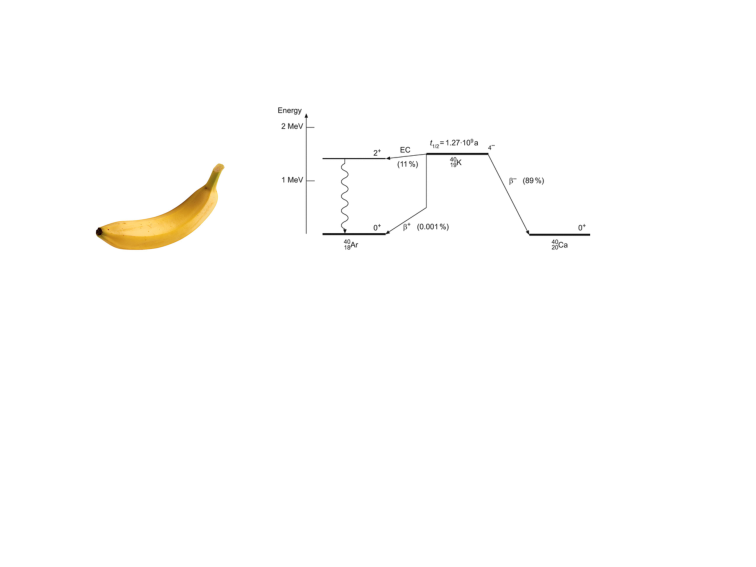
\includegraphics[scale=1.5]{/decadimento_potassio_banane_equivalenti}
\caption{Decadimento del Potassio-40}
\end{figure}

Qual è l'attività di $\SI{1}{g}$ di $K$ naturale?
In un grammo ci sono $N_K = \frac{\SI{1}{g}}{40} \cdot \SI{6.023e23}{} = \SI{1.5e22}{atomi}$ di cui di Potassio-40 
$ N_{^{40}K} = \SI{1.5e22}{} \cdot \SI{1.2e-4}{} = \SI{1.8e18}{atomi} $.
L'attività di $\SI{1}{g}$ di Potassio naturale è pari a
\begin{equation}
A = \frac{dN}{dt} = \lambda N = \frac{\ln 2}{T_{1/2}} = \frac{0.693}{\SI{4e16}{}} = \SI{1.8e18}{} = \SI{31}{Bq}
\end{equation}
in una persona adulta ci sono $\SI{2.5}{g/kg}$ di Potassio, per cui in una persona di $\SI{75}{kg}$ ci sono $\SI{187.5}{g}$ di Potassio e quindi, rispetto al conto precedente, l'attività totale equivale a circa $\SI{5800}{Bq}$.
È da notare che nel corpo umano esistono meccanismi di recupero di questi decadimenti, le cellule sono abituate a recuperare da questo grado di danneggiamento biologico.


\subsubsection{Quantificare danni di eventi disastrosi}
Si quantificano i danni di eventi disastrosi come quelli di Chernobyl facendo una media sulla popolazione.
Noto che una dose di $\SI{1}{Gy}$ è una dose mortale per una persona.
Sapendo la quantità totale di radiazione emessa nell'evento è possibile "dividerla" rispetto alla popolazione per trovarne una media.
Quindi per esempio una dose di $\SI{1}{Gy}$ divisa per $\SI{1000}{persone}$, 1 persona su mille muore per radiazione.

Una dose letale di radiazione espressa in Banane Equivalenti è $\SI{80e6}{BED}$ (lol).

Dormendo a fianco di una persona si è esposti ad una dose di $\SI{0.5}{BED}$.


\subsection{Decadimento $\alpha$}
Nel 1909 Rutherford studia con l'utilizzo di una \emph{camera a nebbia}, uno dei primi rivelatori di particelle, il decadimento nel vuoto di materiale radioattivo e osserva che viene "prodotto" $He$, che osservò come tracce bianche lasciate dal passaggio delle particelle.
Il decadimento $\alpha$ si generalizza come segue
\begin{equation}
\label{decadimento_alpha}
^{A}_{Z}X \quad\rightarrow\quad ^{A-4}_{Z-2}Y + ^{4}_{2}He \quad \Bigl[  + Q  \Bigr]
\end{equation}
in cui il termine $Q$ rappresenta l'energia rilasciata sotto forma di calore.
L'energetica (si chiama così?) del decadimento si calcola, attraverso la solita formula semi-empirica di massa, 
\begin{equation}
Q = M(A,Z) - M(A-4,Z-2) - M_{\alpha}(4,2) = BE(Z-2,A-4) + B_{\alpha} - B(Z,A)
\end{equation}
Se si analizza l'andamento di questa energia in funzione del numero di massa, utilizzando un programma apposito, si trova un andamento del tipo
\begin{figure}[h]
\centering
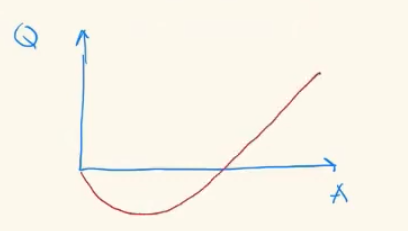
\includegraphics[scale=0.6]{/q_a_alpha}
\caption{CAPTION}
\end{figure}
Il \emph{nucleo di soglia} dal quale il decadimento ha $Q > 0$ corrisponde al numero atomico $A = 150$, quindi gli elementi dal $6^o$ periodo in poi possono decadere $\alpha$, salvo eccezioni come ad esempio l'oro $^{197}_{79}Au$ per il quale nonostante l'energetica sia favorevole al decadimento tale elemento decade con tempi lunghi, più lunghi della vita dell'universo.

\paragraph{Fenomenologia del decadimento alpha} Rappresentando il tempo di decadimento $T_{1/2}$ in funzione dell'energia delle particelle emesse $E_{\alpha}$ si nota una relazione inversa tra le due grandezze, più precisamente data da
\begin{equation}
T_{1/2} \propto \frac{1}{\sqrt{E_{\alpha}}}
\end{equation}
\begin{figure}[h]
\centering
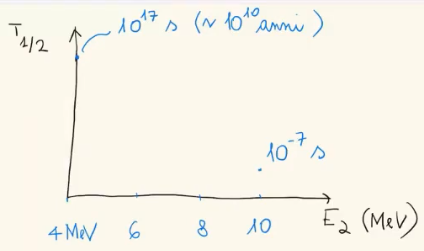
\includegraphics[scale=0.6]{/prop_vitamedia_energiaalpha}
\caption{CAPTION}
\end{figure}
La \emph{legge di Geiger Nuttal} lega la grandezza teorica della \emph{probabilità di decadimento} con le grandezze sperimentalmente misurabili come la \emph{vita media} o il \emph{tempo di dimezzamento}
\begin{equation}
\ln \Bigl(  \frac{1}{\tau}  \Bigr) = a - b \frac{Z}{\sqrt{E_{\alpha}}}
\end{equation}
tale legge ha una validità di $20$ ordini di grandezza, che fa intuire vi siano effetti relativistici che la regolano.

Esistono quattro catene di decadimento alpha molto importanti:
\begin{enumerate}
\item Serie dell'Uranio (o del radio) $^{238}U$ che ha un tempo di vita medio di  $T_{1/2}=\SI{4.5e9}{anni}$ e decade in Piombo $^{206}_{82}Pb$

\item Serie dell'Attino $^{235}U$ che ha un tempo di vita medio di  $T_{1/2}=\SI{7e8}{anni}$ e decade in Piombo $^{207}_{82}Pb$

\item Serie del Torio $^{232}_{90}Th$ che ha un tempo di vita medio di  $T_{1/2}=\SI{1.4e10}{anni}$ e decade in Piombo $^{208}_{82}Pb$

\item Serie del Nettunio $^{237}_{93}Np$ che ha un tempo di vita medio di  $T_{1/2}=\SI{2.2e6}{anni}$ e decade in Bismuto $^{209}_{83}Bi$
\end{enumerate}
Le catene di decadimento vengono utilizzate, tra le altre cose, per le datazioni.
Le precedenti quattro ed il decadimento del Potassio-40 e del Carbonio-14 sono le uniche reazioni di decadimento naturali ancora presenti sulla Terra.
\begin{figure}[h]
\centering
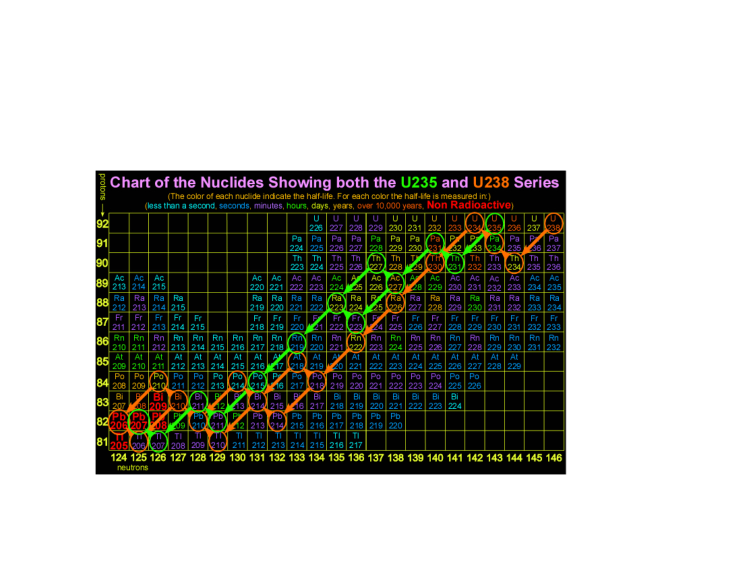
\includegraphics[scale=1.6]{/serie_decadimenti_alpha}
\caption{Serie di decadimenti nucleari dell'Uranio-235 e dell'Uranio-238, in cui si alternano decadimenti $\alpha$ e $\beta$}
\end{figure}

Studiamo il decadimento di un nucleo padre $X$ che decade in un nucleo figlio $Y$ più una particella $\alpha$ ed energia $Q$
\begin{equation}
^{A}_{Z}X \quad\rightarrow\quad ^{A-4}_{Z-2}Y + ^{4}_{2}He + Q
\end{equation}
se inizialmente l'atomo $X$ è a riposo, per la conservazione della quantità di moto, i figli di questa reazione si allontaneranno in direzioni opposte.
La conservazione della quantità di moto si esprime come 
\begin{equation}
p_Y = p_{\alpha} = p
\end{equation}
L'energia liberata nella reazione è divisa tra l'energia cinetica del nucleo figlio e dalla particella $\alpha$, per cui usando la meccanica classica otteniamo
\begin{equation}
Q = \frac{p_Y^2}{2m_Y} + \frac{p_{\alpha}^2}{2m_{\alpha}} 
= \frac{p^2}{2} \Bigl(  \frac{1}{m_Y}  + \frac{1}{m_{\alpha}}\Bigr)
= \frac{p^2}{2} \Bigl(  \frac{m_Y + m_{\alpha}}{m_Y m_{\alpha}} \Bigr)
\end{equation}
da cui si estrae $p^2$
\begin{equation}
p^2 = 2 Q \Bigl(  \frac{m_Y m_{\alpha}}{m_Y + m_{\alpha}} \Bigr)
\end{equation}
da cui si trova come si distribuisce l'energia cinetica nella reazione, l'energia cinetica della particella $\alpha$ è
\begin{equation}
K_{\alpha} = \frac{p^2}{2m_{\alpha}} = Q \frac{m_Y}{m_Y + m_{\alpha}}
\end{equation}
e.g. per un atomo che decade alpha con un numero di massa $A = 200$, sapendo che $A_{\alpha} = 4$ si trova
\begin{equation}
K_{\alpha} = Q \frac{196}{200} \simeq 98\% Q
\end{equation}
e quindi praticamente tutta l'energia cinetica viene trasferita alla particella, mentre solo un $2\%$ dell'energia cinetica viene trasferita all'atomo figlio.
Ha senso quindi approssimare dicendo che l'energia rilasciata nella reazione equivale (circa) all'energia cinetica della particella alpha e quindi si può scrivere $K_{\alpha} = Q$.

\paragraph{nota} se nel decadimento (a due corpi) fosse emesso un elettrone allora l'energia cinetica dell'elettrone sarebbe $K_e = 0.999 Q$

\subsubsection{Cos'è il decadimento $\alpha$}
In un nucleo con massa atomica sufficientemente alta c'è una probabilità non nulla che si formi una particella $\alpha$, un nucleo di Elio, al suo interno, questa particella iniziando a rimbalzare all'interno del nucleo arriverà sulle "pareti".
Il potenziale nucleare è composto da una buca di potenziale che oltre il confine decresce esponenzialmente, l'energia della particella alpha equivale a $E_{\alpha} = \SI{28}{MeV}$.
L'emissione diretta di protoni e neutroni non è possibile in quanto la loro energia $E= 7-\SI{8}{MeV}$ si trova al disotto del livello zero dell'energia e sono intrappolati all'interno.
\begin{figure}[h]
\centering
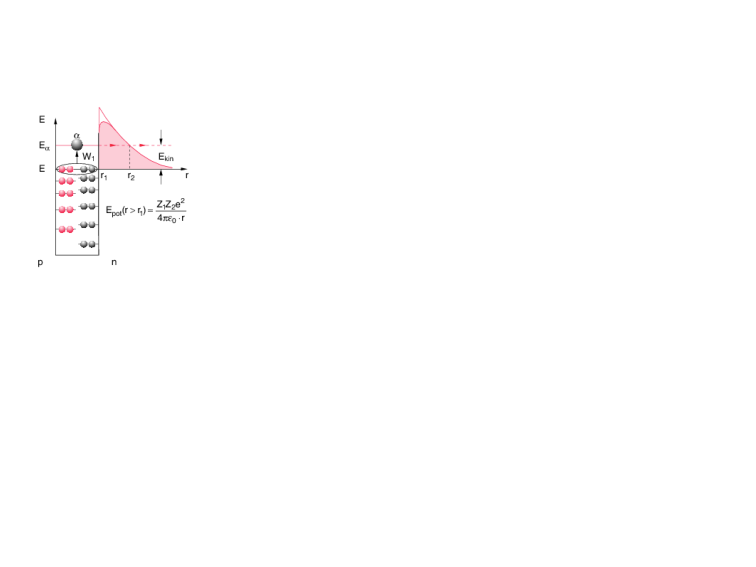
\includegraphics[scale=2]{/alpha_decad_potenziale}
\caption{CAPTION}
\end{figure}
Se i protoni ed i neutroni si combinano insieme in una particella $\alpha$, particella molto stabile, viene emessa un'energia maggiore del livello zero, per cui è inizialmente intrappolata nella buca di potenziale ma ha una probabilità di uscire dalla buca diversa da zero.
Ovviamente solo per effetti quantistici la particella potrà attraversare la regione di potenziale maggiore dell'energia $E_{\alpha}$, classicamente il decadimento $\alpha$ non è possibile o spiegabile.

Cerco qual è la barriera di potenziale che la particella deve superare.
Chiamando $r_1$ la distanza in cui si trova il picco più alto di potenziale, quindi sulla superficie del nucleo, e.g. calcolato per l'Uranio-238 trovo
\begin{equation}
\begin{split}
r_1 & = 1.2 ( 234^{1/3} + 4^{1/3} ) = \SI{9.3}{fm} \\
V_1 & = \frac{ Z_Y \cdot Z_{He} e^2}{4 \pi \varepsilon_0 r_1} = \frac{ 90 \cdot 2 e^2}{4 \pi \varepsilon_0 r_1} = \frac{180 e^2 \hbar c }{4 \pi \varepsilon_0 \hbar c r_1} = \frac{180 \cdot \SI{1.44 }{MeV fm}}{ \SI{9.3}{fm} } =  \SI{27.8}{MeV} 
\end{split}
\end{equation}
La particella $\alpha$ pur avendo energia positiva è inferiore al valore del potenziale, poiché è dell'ordine di qualche $MeV$. 

Cerco ora la distanza che la particella deve percorrere per \emph{effetto tunnel} fino al punto $r_2$ in cui l'energia del potenziale è uguale all'energia della particella $\alpha$.
Per questo conto teniamo ancora in considerazione l'Uranio, l'energia della reazione equivale ad $E_{\alpha} = Q = \SI{4.2}{MeV}$ ed eguagliandolo al potenziale dell'atomo si ricava
\begin{equation}
\begin{split}
& Q = V = \frac{1}{4 \pi \varepsilon_0} \frac{90\cdot2}{r_2} \\
& r_2 = \frac{180 \cdot \SI{1.44}{MeV fm}}{\SI{4.2}{MeV}} = \SI{61.7}{fm}
\end{split}
\end{equation}
La barriera che la particella deve attraversare è molto profonda e non è per questo molto probabile che succeda.


\subsubsection{Teoria di Gamov del decadimento $\alpha$}
La vita media del decadimento è inversamente proporzionale alla probabilità
\begin{equation}
\tau = \frac{1}{\lambda}
\end{equation}
il tempo di decadimento è un parametro fenomenologico, sperimentale, mentre la probabilità di decadimento si ricava dalla teoria.
Secondo la \emph{teoria di Gamov} la probabilità di decadimento è data da tre contributi:
\begin{equation}
\lambda = p_{\alpha} f P
\end{equation}
in cui
\begin{itemize}
\item $p_{\alpha}$ è la \emph{probabilità che si formi una particella $\alpha$}

\item $f$ è la \emph{frequenza di collisione} tra la particella $\alpha$ e gli altri nucleoni nel nucleo ovvero posta $v_{\alpha}]$ la velocità della particella nel nucleo ed $r_1$ la dimensione del nucleo, si ha 
\begin{equation}
\begin{split}
& f = \frac{v_{\alpha}}{2 r_1} \\
& v_{\alpha} = \sqrt{ 2\frac{V_0 + Q}{m_{\alpha}} } \simeq \sqrt{ 2\frac{\SI{35}{MeV} + \SI{5}{MeV}}{\SI{3700}{MeV/c^2}} } \simeq \SI{0.14}{c} = \SI{0.42e8}{m/s}
\end{split}
\end{equation}
considerando ad esempio un nucleo con $A=200$ e raggio $R = \SI{7.0}{fm}$, si trova una frequenza di $f = \SI{6e21}{Hz}$, quindi molto alta

\item mentre il parametro $P$ è legato alla \emph{probabilità di attraversamento della barriera di potenziale}, per il quale è necessario applicare l'equazione di Schrodinger indipendente dal tempo.
Considero il potenziale nella zona 2, in cui decresce da $r_1$ a $r_2$.
Data l'equazione di Schrodinger
\begin{equation}
\begin{split}
-\frac{\hbar^2}{2m} \frac{d^2 \psi}{dx^2} V \psi = E \psi \quad\Rightarrow\quad 
& \frac{d^2\psi}{dx^2} = - \frac{2m}{\hbar^2} (E-V)\psi = -\frac{2m}{\hbar^2} (Q-V_c)\psi \\
K^2 =  -\frac{2m}{\hbar^2} (Q-V_c) \quad > 0 & \\
&  \frac{d^2\psi}{dx^2} = K^2 \psi \quad\Rightarrow\quad \psi = \cancel{A e^{+ K x}} + Be^{- K x}
\end{split}
\end{equation}
si trova la funzione d'onda $\psi$ che descrive la particella nella zona classicamente proibita.
Il valore di $K^2$ trovato nella formula precedente è sempre positivo ed è l'argomento dell'esponenziale.
Se $Q \ll V_c$ mi aspetto che l'esponenziale abbia un andamento molto rapido di decadimento, se invece $Q \sim V_c$ il decadimento esponenziale è molto più lento, vedi figura \ref{decad_q_Vc}.
\begin{figure}[h]
\centering
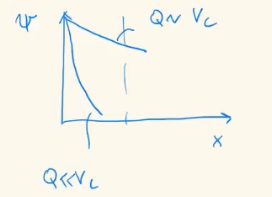
\includegraphics[scale=0.7]{/esp_Q_Vc}
\caption{dipendenza tra il decadimento e l'energia}
\label{decad_q_Vc}
\end{figure}
Esiste quindi una grande dipendenza tra la vita media ed il gradino di potenziale da dover superare e quindi dall'energia emessa dalla reazione.
\end{itemize}

\paragraph{Calcolo del potenziale da attraversare con effetto tunnel}
Il potenziale $V$ è composto da due zone distinte, la prima tra lo zero ed il valore $R$ del raggio del nucleo il potenziale è costituito da una buca $V=V_0$, mentre la seconda zona, da $R$ in poi, è dato dal potenziale coulombiano $V=V_c(r)$, per cui 
\begin{equation}
V(r) =
\Bigg\{\begin{array}{l}
\mbox{se}\quad r \in [ 0, R ] \quad\Rightarrow\quad  V_0  \\
\mbox{se}\quad r \in [ R, \infty [ \quad\Rightarrow\quad \frac{2(Z-2)e^2}{4 \pi \varepsilon_0} \frac{1}{r} 
\end{array}
\end{equation}
Il parametro $K$ è ciò che dobbiamo considerare per lo studio dell'andamento della probabilità $e^{-2 G}$
\begin{equation}
K(r) = \sqrt{ \frac{2m}{\hbar^2} \Bigl(  V_c(r) -Q \Bigr) } = \sqrt{ \frac{2m}{\hbar^2} \frac{2(Z-2)e^2}{4 \pi \varepsilon_0} \Bigl(  \frac{1}{r} - \frac{1}{b}  \Bigr) } 
\end{equation}
per cui lo integriamo tra $R$ e $b$, in cui il potenziale vale $V_c(b) = \frac{2(Z-2)e^2}{4 \pi \varepsilon_0} \frac{1}{b}$, per ottenere il primo risultato del fattore di Gamov $G$
\begin{equation}
\begin{split}
G & = \sqrt{ \frac{2m}{\hbar^2} \frac{2(Z-2)e^2}{4 \pi \varepsilon_0} } \int_R^{b} \sqrt{ \frac{1}{r} - \frac{1}{b}  } dr \\
& \mbox{sostituisco} \quad r = b \sin^2 \theta \quad\Rightarrow\quad dr = 2b \sin \theta \cos \theta d\theta \\
& = \sqrt{ \frac{2m}{\hbar^2} \frac{2(Z-2)e^2}{4 \pi \varepsilon_0} } \int_{\sin^{-1}\sqrt{\frac{R}{b}}}^{\pi/2} 2 \sqrt{b} \cos^2 \theta d\theta \\ 
& = \sqrt{ \frac{2m}{\hbar^2} \frac{2(Z-2)e^2}{4 \pi \varepsilon_0} } \sqrt{b} \int_{\sin^{-1}\sqrt{\frac{R}{b}}}^{\pi/2} \Bigl(  1 + \cos(2\theta)  \Bigr) d\theta \\
& = \sqrt{ \frac{2m}{\hbar^2} \frac{2(Z-2)e^2}{4 \pi \varepsilon_0} } \sqrt{b} \Bigl[  \theta + \frac{1}{2}\sin(2\theta)  \Bigr]_{\sin^{-1}\sqrt{\frac{R}{b}}}^{\pi/2} \\
& =\sqrt{ \frac{2m}{\hbar^2} \frac{2(Z-2)e^2}{4 \pi \varepsilon_0} } \sqrt{b} \Bigl[  \cos^{-1}\sqrt{\frac{R}{b}} - \sqrt{\frac{R}{b}\Bigl(  1- \frac{R}{b}   \Bigr)} \Bigr]
\end{split}
\end{equation}
Esplicitiamo ora i termini $R, b$
\begin{equation}
\begin{split}
& B = \frac{2 (Z-2) e^2}{4 \pi \varepsilon_0 R} \quad\Rightarrow\quad R = \frac{2 (Z-2) e^2}{4 \pi \varepsilon_0 B} \\
& Q_{\alpha} = \frac{2 (Z-2) e^2}{4 \pi \varepsilon_0 b} \quad\Rightarrow\quad b = \frac{2 (Z-2) e^2}{4 \pi \varepsilon_0 Q_{\alpha}} 
\end{split}
\end{equation}
e riscriviamo il fattore di Gamov
\begin{equation}
\begin{split}
G &= \frac{2 (Z-2) e^2}{4 \pi \varepsilon_0 \hbar} \sqrt{\frac{2m}{Q_{\alpha}}} \Bigl[  \cos^{-1}\sqrt{\frac{Q_{\alpha}}{B}} - \sqrt{\frac{Q_{\alpha}}{B} \Bigl(  1 - \frac{Q_{\alpha}}{B}  \Bigr)}  \Bigr] \\
& \quad\quad x=\frac{Q_{\alpha}}{B} \quad\mbox{per $x$ piccoli}\quad \cos^{-1}x \sim \frac{\pi}{2} - x \\
& = \frac{2 (Z-2) e^2}{4 \pi \varepsilon_0 \hbar} \sqrt{\frac{2m}{Q_{\alpha}}} \Bigl[  \frac{\pi}{2} - 2 \sqrt{\frac{Q_{\alpha}}{B}}  \Bigr]
\end{split}
\end{equation}
il potenziale a raggio $R$ vale $B$, ovvero
\begin{equation}
V(R) = B = \frac{2 (Z-2) e^2}{4 \pi \varepsilon_0 R} = \frac{2 Z_d e^2}{4 \pi \varepsilon_0 R}
\end{equation}
dove $Z_d$ è il numero di protoni del nucleo figlio.
La probabilità di attraversamento per effetto tunnel è
\begin{equation}
\begin{split}
P = e^{-2 G} \quad\Rightarrow\quad \ln P &= -2 G \\
& = -\frac{e^2}{\varepsilon_0 \hbar} \sqrt{\frac{m}{2}} Z_d \frac{1}{\sqrt{Q_{\alpha}}} + \frac{4 e}{\hbar} \sqrt{\frac{m}{\pi \varepsilon_0}} \sqrt{Z_d} \sqrt{R} \\ 
& \quad\mbox{sostituendo}\quad R = R_0 A^{1/3} \\
log_{10} P = & 1.42 \sqrt{Z_d A^{1/3}} - 1.72 \frac{Z_d}{\sqrt{Q_{\alpha}}}
\end{split}
\end{equation}
il primo termine è pressoché costante, mentre è il secondo termine ad avere l'impatto maggiore.

\subsubsection{Applicazione del decadimento $\alpha$}
\paragraph{Generatore elettrico}
Il rover \emph{Perserverance} mandato su Marte viene alimentato grazie a delle sorgenti $\alpha$, il Plutonio-238.
Il $^{238}Pu$ ha un tempo di dimezzamento $T_{1/2} \simeq \SI{88}{y}$ ed il decadimento produce calore che per \emph{Effetto Seebeck} viene convertito in elettricità.

Calcoliamo l'energia rilasciata da $\SI{238}{g}$ di $^{238}Pu$, quindi l'attività $A$ è
\begin{equation}
\begin{split}
A & = N_0 \lambda = \frac{\SI{238}{g}}{238} \SI{6.023e23}{} \frac{0.693}{90 \cdot 365 \cdot 25 \cdot 3600} \\
& \SI{1.5e14}{\frac{decadimenti}{s}}
\end{split}
\end{equation}
l'energia della singola particella $\alpha$ è
\begin{equation}
Q_{\alpha} = E_{\alpha} \Bigl(  \frac{M_{\alpha}+M_d}{M_{\alpha} M_d}  \Bigr) = \SI{5.6}{MeV}
\end{equation}
e l'energia totale rilasciata è 
\begin{equation}
E = A \cdot Q_{\alpha} = \SI{1.5e14}{s^{-1}} \SI{5.6}{MeV} = \SI{e14}{MeV/s} \cdot \SI{1.6e-19}{MeV} = \SI{1.4e2}{W}
\end{equation}
questa grandezza esprime $joule$ termici rilasciati, quelli poi convertiti in elettricità saranno solo una frazione di questi, ma l'efficienza di conversione è abbastanza bassa per questo tipo di generatore e servono alcuni $kg$ di Plutonio per renderli utilizzabili.
   
\paragraph{Datazione della Terra} 
Sfruttiamo il processo di decadimento dell'Uranio-238 in Piombo-206. 
Le pietre più antiche sulla terra sono gli \emph{zirconi}, esse preservano al loro interno i composti chimici salvaguardandoli da alterazioni geologiche, chimiche e nel tempo. 
Analizzando la composizione chimica interna di uno zircone e cercando le quantità di Uranio-238 e di Piombo-206 è possibile risalire ad una età di tale zircone; in quanto si ipotizza (e si conosce) che il Piombo deriva unicamente dal decadimento dell'Uranio.

Anche i \emph{meteoriti} forniscono molte informazioni sull'età della Terra, essi sono "capsule del tempo" che ci permettono di osservare la composizione del sistema solare al momento della sua formazione e quindi di fare un paragone con i composti presenti oggi sulla Terra.
Al contrario, la Terra è sempre in cambiamento, quindi non è facile trovare campioni antichi quanto la formazione su di essa.

\subsection{Decadimento $\beta$}
I nuclei decadono $\beta$ tendono ad avvicinarsi alla valle di stabilità del grafico dei nuclei $Z-N$ e decadono $\beta$ quei nuclei che hanno troppi protoni $(\beta^+)$ o troppi neutroni $(\beta^-)$.


\paragraph{Decadimento $\beta^+$} il nucleo può avere troppi protoni, si ha allora un processo di decadimento beta $\beta^+$
\begin{equation}
^{A}_{Z}X \quad\longrightarrow\quad ^{A}_{Z-1}Y + e^+ + \nu_e
\end{equation}
dopo il decadimento si ha un atomo di una diversa specie atomica.
Nel dettaglio vediamo che questo processo è descritto dal decadimento di un protone
\begin{equation}
p \quad\longrightarrow\quad n + e^+ + \nu_e
\end{equation}
e a livello di quark 
\begin{equation}
u \quad\longrightarrow\quad d + e^+ + \nu_e
\end{equation}
Il bilancio energetico 
\begin{equation}
Q = M(A,Z) - M(A,Z+1) - m_e > 0
\end{equation}


\paragraph{Decadimento $\beta^-$}  il nucleo ha troppi neutroni, allora si ha un processo di decadimento beta $\beta^-$
\begin{equation}
^{A}_{Z}X \quad\longrightarrow\quad  ^{A}_{Z+1}Y + e^- + \bar\nu_e
\end{equation}
dopo il decadimento si ha un atomo della stessa specie X.
Questo processo è descritto in dettaglio da un decadimento di un neutrone
\begin{equation}
n \quad\longrightarrow\quad p + e^- + \bar\nu_e
\end{equation}
a livello di quark tale processo consiste nella conversione di un quark down in un quark up
\begin{equation}
d \quad\longrightarrow\quad u + e^- + \bar\nu_e
\end{equation}
mediato dal bosone $W$, mediatore della forza debole.
Il decadimento si verifica quando il calore $Q$ della reazione è maggiore di zero, per cui calcolo la differenza tra la massa iniziale e finale che corrisponde all'energia emessa o assorbita,
\begin{equation}
Q = M(A,Z) - M(A,Z+1) - m_e > 0
\end{equation}

















